\documentclass[a4paper,12pt]{article}
\usepackage[T2A]{fontenc}
\usepackage[utf8]{inputenc}
\usepackage[russian]{babel}
\usepackage{amsmath}
\usepackage{graphicx}
\usepackage{float}
\usepackage{indentfirst}
\usepackage[left=2.5cm,right=1.5cm,top=2cm,bottom=2cm]{geometry}

\title{Численные методы решения дифференциальных уравнений}
\author{Студент группы 251\\
Факультет КНиИТ}
\date{2024}

\begin{document}

\maketitle

\tableofcontents
\newpage

\section*{Введение}
\addcontentsline{toc}{section}{Введение}

В данной работе рассматриваются численные методы решения обыкновенных дифференциальных уравнений: метод Эйлера и метод Рунге-Кутты 4-го порядка.

\section{Постановка задачи}

Рассмотрим задачу Коши:

\begin{equation}
    \frac{dy}{dt} = f(t, y), \quad y(t_0) = y_0 \label{eq:cauchy}
\end{equation}

В качестве тестового примера возьмём уравнение:

\begin{equation}
    \frac{dy}{dt} = y - t^2 + 1, \quad y(0) = 0.5 \label{eq:example}
\end{equation}

Аналитическое решение:

\begin{equation}
    y(t) = (t+1)^2 - 0.5e^t \label{eq:exact}
\end{equation}

\section{Метод Эйлера}

Формула метода:

\begin{equation}
    y_{n+1} = y_n + h \cdot f(t_n, y_n) \label{eq:euler}
\end{equation}

\section{Метод Рунге-Кутты 4-го порядка}

\begin{equation}
    \begin{aligned}
    k_1 &= f(t_n, y_n) \\
    k_2 &= f(t_n + \frac{h}{2}, y_n + \frac{h}{2}k_1) \\
    k_3 &= f(t_n + \frac{h}{2}, y_n + \frac{h}{2}k_2) \\
    k_4 &= f(t_n + h, y_n + h k_3) \\
    y_{n+1} &= y_n + \frac{h}{6}(k_1 + 2k_2 + 2k_3 + k_4)
    \end{aligned} \label{eq:rungekutta}
\end{equation}

\section{Программная реализация}

\begin{verbatim}
def f(t, y):
    return y - t**2 + 1

def euler(f, t0, y0, h, n):
    t = [t0]
    y = [y0]
    for i in range(n):
        t.append(t[-1] + h)
        y.append(y[-1] + h * f(t[-2], y[-1]))
    return t, y

def runge_kutta(f, t0, y0, h, n):
    t = [t0]
    y = [y0]
    for i in range(n):
        t.append(t[-1] + h)
        k1 = f(t[-2], y[-1])
        k2 = f(t[-2] + h/2, y[-1] + h/2 * k1)
        k3 = f(t[-2] + h/2, y[-1] + h/2 * k2)
        k4 = f(t[-2] + h, y[-1] + h * k3)
        y.append(y[-1] + h/6 * (k1 + 2*k2 + 2*k3 + k4))
    return t, y
\end{verbatim}

\section{Результаты}

\begin{table}[H]
\centering
\caption{Сравнение методов при h = 0.1}
\begin{tabular}{|c|c|c|c|}
\hline
t & Точное & Эйлер & Рунге-Кутта \\ \hline
0.0 & 0.5000 & 0.5000 & 0.5000 \\
0.5 & 1.4256 & 1.4250 & 1.4256 \\
1.0 & 2.6409 & 2.6390 & 2.6409 \\
1.5 & 4.0092 & 4.0048 & 4.0092 \\
2.0 & 5.3055 & 5.2977 & 5.3055 \\ \hline
\end{tabular}
\end{table}

% Изображения временно закомментированы, так как нет реальных файлов .png
% \begin{figure}[H]
% \centering
% 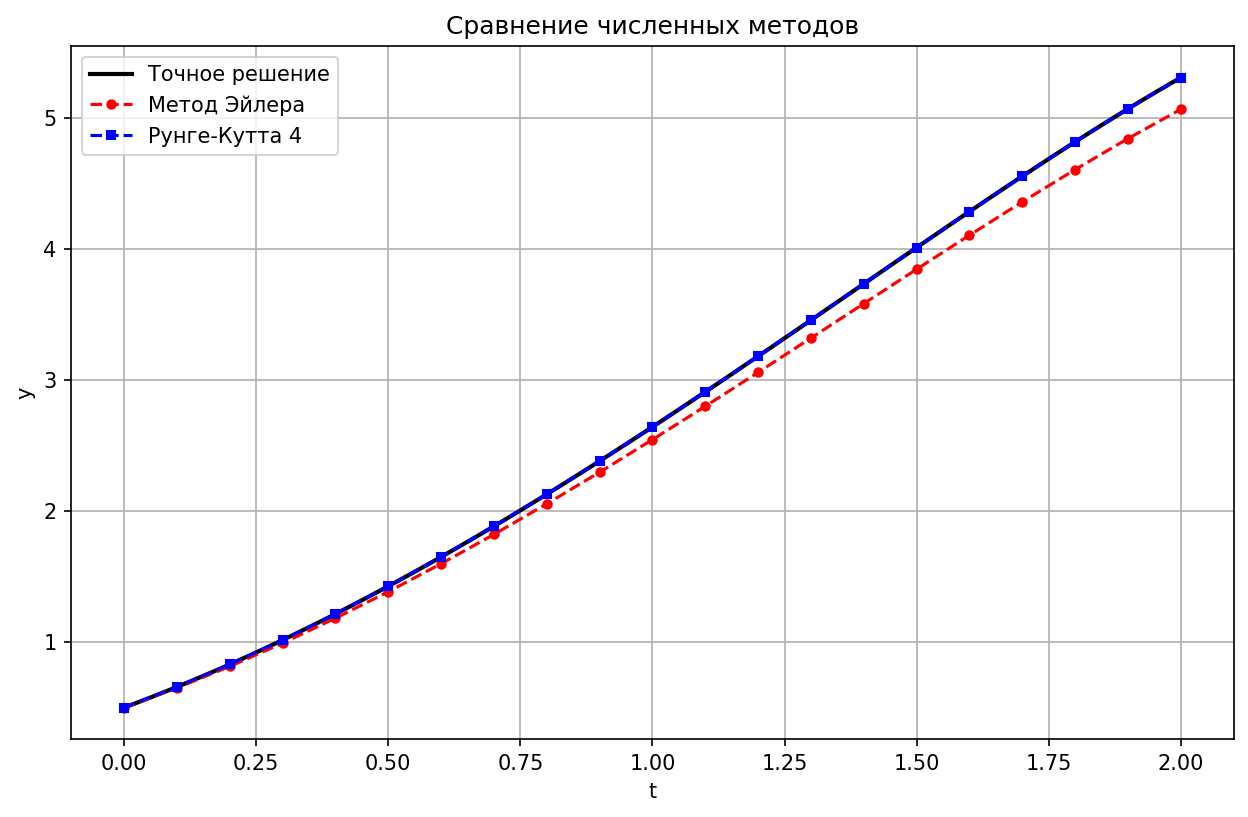
\includegraphics[width=0.7\textwidth]{images/comparison.png}
% \caption{График сравнения методов}
% \label{fig:comparison}
% \end{figure}

% \begin{figure}[H]
% \centering
% \includegraphics[width=0.7\textwidth]{images/error.png}
% \caption{График ошибок}
% \label{fig:error}
% \end{figure}

\section{Заключение}

Метод Рунге-Кутты 4-го порядка показал более высокую точность по сравнению с методом Эйлера.

\bibliographystyle{plain}
\begin{thebibliography}{9}

\bibitem{verma} Verma A. Numerical Methods for Differential Equations. Springer, 2023.

\bibitem{butcher} Butcher J.C. Numerical Methods for Ordinary Differential Equations. Wiley, 2016.

\end{thebibliography}

\end{document}